\documentclass{article}
% General document formatting
\usepackage[margin=0.7in]{geometry}
\usepackage[parfill]{parskip}
\usepackage[utf8]{inputenc}
\usepackage{hyperref} 
\usepackage{booktabs}
\usepackage{graphicx}
\usepackage{subfig}
\usepackage{caption}
\usepackage{fancyhdr}

% Related to math
\usepackage{amsmath,amssymb,amsfonts,amsthm}
\title{Proposal - Playing pokemon battles optimally}
\author{Julian Schubert}

% Kopf- / Fußzeile
\makeatletter
\let\runauthor\@author
\let\runtitle\@title
\pagestyle{fancy}
\fancyhf{}
\rhead{\runtitle}
\lhead{\runauthor}
\cfoot{\thepage}

\begin{document}
\maketitle

\section{Introduction}
Pokemon is a video game series created by the Pokemon Company.
The goal of the game is to not only catch pokemon, but also to train them and use
them to battle other trainers. In the mainline games, the focus lies on the story
as well as exploring the world. The pokemon genere has evolved quite a bit since
it's early days, Figures \ref{fig:red0} and \ref{fig:red1} contain screenshots 
of the first pokemon games, pokemon red and pokemon green.
\begin{figure}[ht]
    \centering
    \begin{minipage}{.5\textwidth}
      \centering
      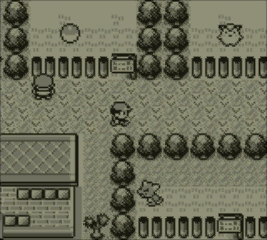
\includegraphics[width=.9\linewidth]{images/Red-0.jpg}
      \captionof{figure}{Exoploring the map in pokemon red}
      \label{fig:red0}
    \end{minipage}%
    \begin{minipage}{.5\textwidth}
      \centering
      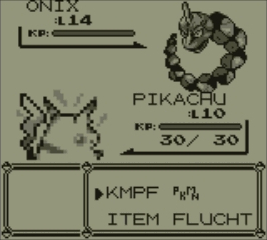
\includegraphics[width=.9\linewidth]{images/Red-1.jpg}
      \captionof{figure}{Fighting another trainer in pokemon red}
      \label{fig:red1}
    \end{minipage}
    \caption*{Image source: \href{https://www.nintendo.de/Spiele/Game-Boy/Pokemon-Rote-Edition-266109.html}{nintendo.de}}
\end{figure}
Figures \ref{fig:sword0} and \ref{fig:sword1} contain ingame footage of the latest games in
the series, pokemon sword and shield.
\begin{figure}
  \centering
  \begin{minipage}{.48\textwidth}
    \centering
    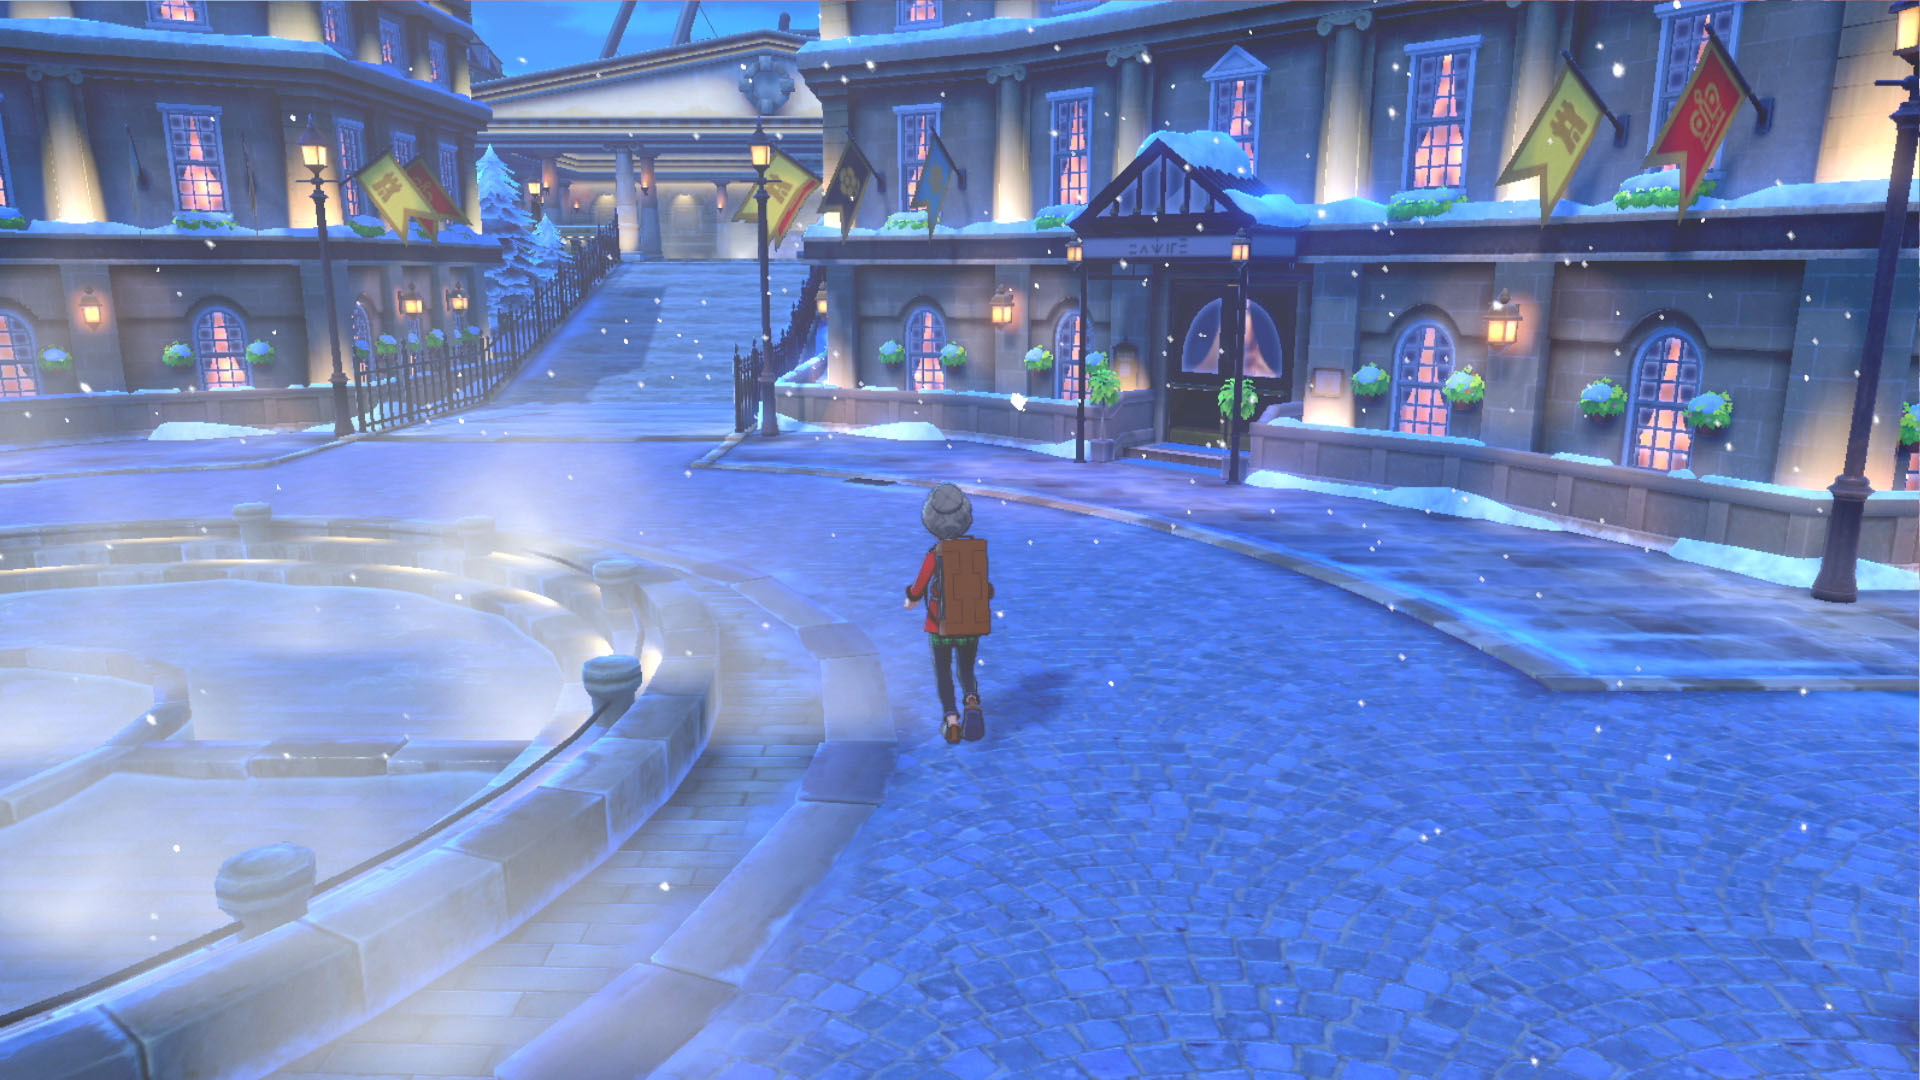
\includegraphics[width=.9\linewidth]{images/Sword-0.jpg}
    \captionof{figure}{Exoploring the map in pokemon sword. \\ 
      Image source: \href{https://swordshield.pokemon.com/de-de/gameplay/pokemon-battle-stadium/}{pokemon.com}}
    \label{fig:sword0}
  \end{minipage}%
  \begin{minipage}{.48\textwidth}
    \centering
    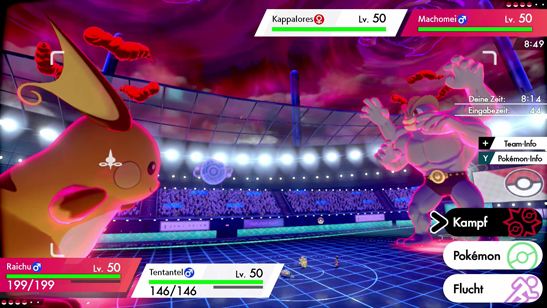
\includegraphics[width=.9\linewidth]{images/Sword-1.jpg}
    \captionof{figure}{Fighting another trainer in pokemon sword \\
      Image source: Image source: \href{https://www.nintendo.de/Spiele/Nintendo-Switch/Pokemon-Schwert-1522111.html}{nintendo.de}}
    \label{fig:sword1}
  \end{minipage}
\end{figure}
This thesis will exclusivly focus exclusivly on battling as there detailed lists
of the locations of everything there is to explore within the games.

\section{Prerequisites}
Nintendo does not provide an API for the game, however, the fan project
\href{https://play.pokemonshowdown.com/}{Pokemon Showdown} is a
free online tool that can be used to battle online trainers. On top of that,
it provides the functionality to use their simulator offline in an CLI. The
entire source code for pokemon showdown can be found at 
\href{https://github.com/smogon/pokemon-showdown}{Github}.
Additionally, the python library \href{https://poke-env.readthedocs.io/en/latest/}{poke-env}
is used as it provides a convenient interface to showdown. \\
The combination of both tools allows to easily perform deep reinforcement learning
on a local running instance of showdown, as well as evaluating models against 
human players on the official pokemon showdown server. Figure \ref{fig:showdown-battle}
shows a battle between two human players on pokemon showdown. Lastly, the creators
of pokemon showdown provided me with over 8 Million replays of games played
by humans.

\section{Battling}
There are multiple popular battle formats in pokemon as well as in pokemon
showdown. This research will focus exclusively on the most popular category
on showdown: Random battles with pokemon from all differnet games. \\
\textit{Note:} In the mainline games items also play a huge role in battle,
as they for example allow the revival of a fainted pokemon. In competive
play items are banned, only held items allowed. A held item can for example
allow a pokemon to more often be able to attack first or trade in defensive
stats for offensive ones.

\subsection{Fundamentals}
At the start of the game, each player gets 6 different random pokemon. A player
knows all 6 pokemon he has with all their available moves, yet, he only knows
the active pokemon of his opponent. Additionally, the player does not know what
moves the opposing pokemon is able to use. Each pokemon knows 4 different moves,
a move can either \textit{attack}, \textit{strengthen} himself or the own team,
or \textit{weaken} the enemy pokemon or team by for example poisoning the enemy
pokemon. \\ 
Pokemon battles are turn based, each turn, both players either choose a move
for their active pokemon, or switch to another pokemon of the team. 

\subsection{Type advantages}
\begin{figure}[ht]
  \centering
  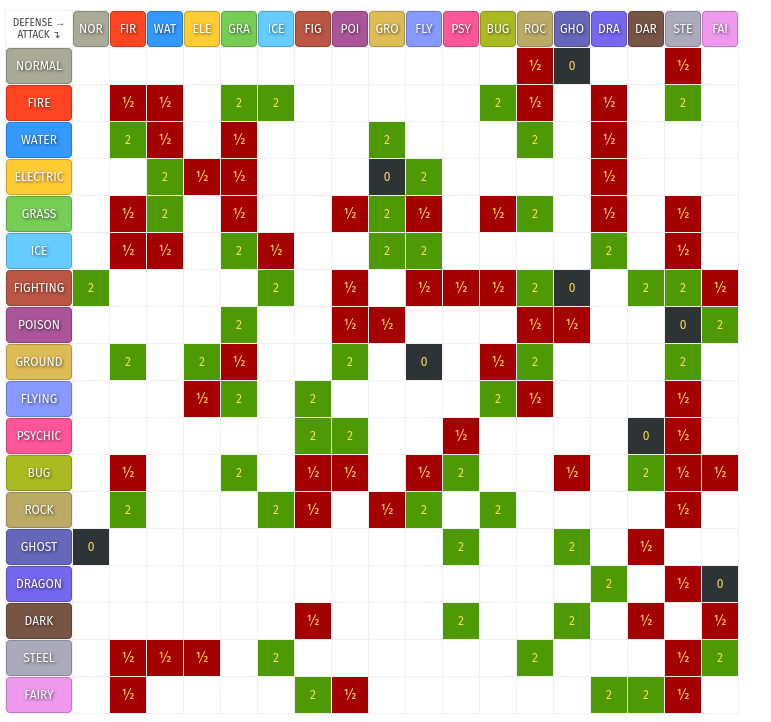
\includegraphics[width=.9\linewidth]{images/Types.png}
  \captionof{figure}{Type chart \\
    Image source: \href{https://pokemondb.net/type}{pokemondb.net}}
  \label{fig:type-chart}
\end{figure}
The game works implements rock-paper-scissors-like system. Each pokemon has one
or two types, each move has a type as well. A pokemon has a \textit{type advantage}
against an other pokemon, if his moves deal extra damage againt the opposing pokemon.
Figure \ref{fig:type-chart} shows how every type interacts with every other type.
For example, a \textbf{Fire} deals normal damage against \textbf{Electric}, twice
as much damage against \textbf{Bug} and only the half amount of damage against
\textbf{Rock}. \\
\textit{Note:} These damage modifiers are multiplied with each other, so if a 
fire move were to hit a pokemon with type electric and bug, the move would
deal the usual amount of damage.

\subsection{Showdown battle interface}
Figure \ref{fig:showdown-battle} is taken from an ongoing battle on pokemon
showdown. The red marking shows the remaining hit points (hp) player ones
active pokemon. As the bar is completely full, the pokemon still has 
not taken any damage. Once a pokemon has no health remaining, it faints,
and the player has to switch to another pokemon. 
The enemy pokemon
only has 33\% of its health remaining. As highlighted by the green 
marking, the enemy pokemon is called "Kommo-o", is male and has
level 80. In the blue marked are the status affects displayed. For
example, the attack-stat of "Kommo-o" is raised by 50\%. Framed
yellow is the team oft the opposing player. Both grayed out
pokemon are fainted and therfore can't be send into battle,
the fully colored pokemon are still alive and the ball in
the bottom right corner indicates one unknown pokemon the 
player hasn't sent out yet. \\
Below that, the four moves the mewto can pick from are displayed.
In this case, these moves are \textbf{Fire Blast}, \textbf{Recover},
\textbf{Psystrike} and \textbf{Nasty Plot}.

\begin{figure}[ht]
  \centering
  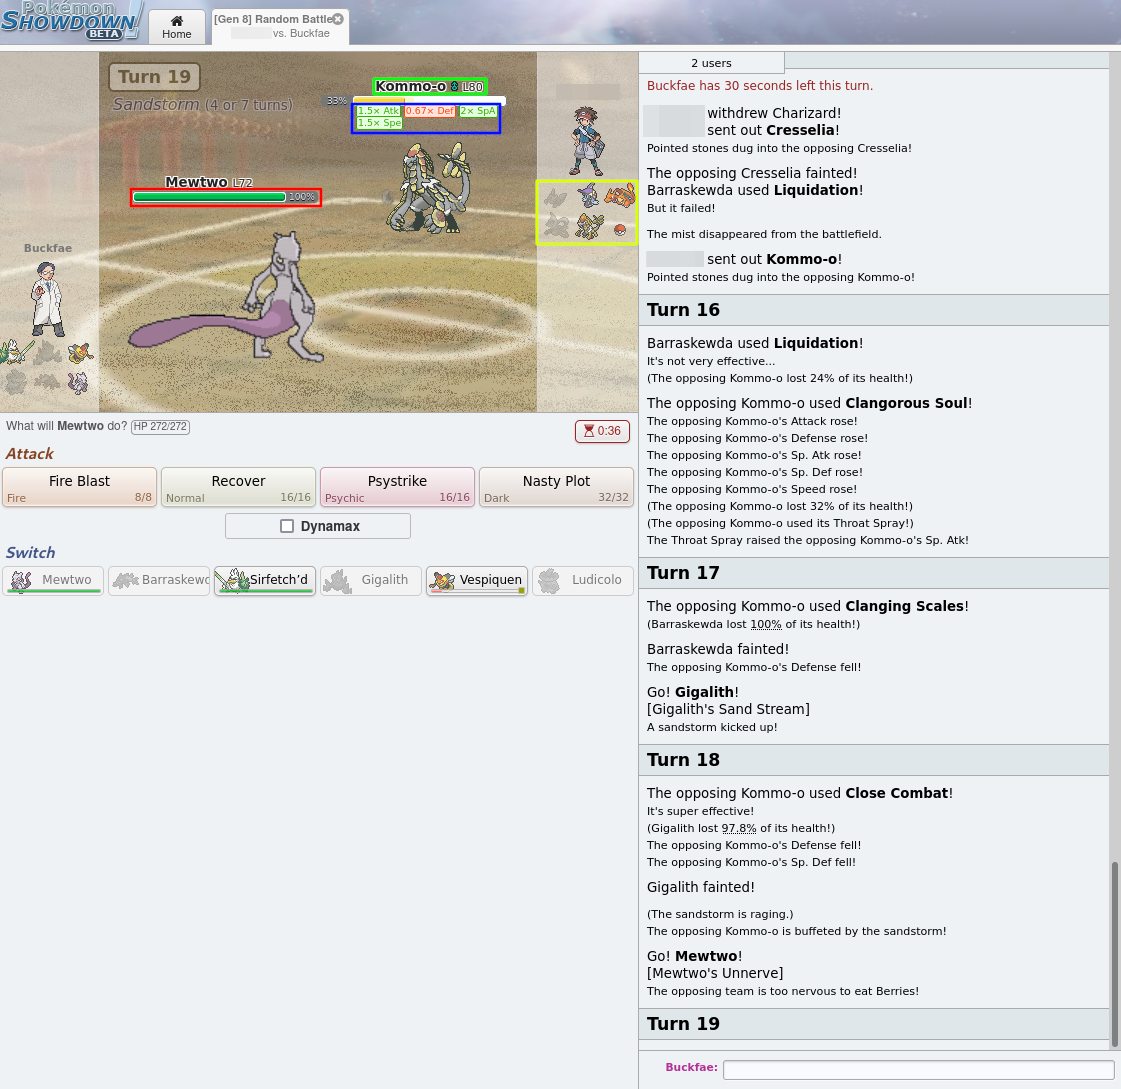
\includegraphics[width=.9\linewidth]{images/Showdown.png}
  \captionof{figure}{Screenshot of me batteling a random opponent}
  \label{fig:showdown-battle}
\end{figure}

\subsection{Advanced battling strategies}
In section \ref{sec:rulebased} a simpe rulebased approach is introduced that 
always picks the move that deals the most amount of damage. However, picking 
an optimal move is a lot more complex than this. Pokemon battles are not just
strict one on one battles where the player with the most damage dealing pokemon
always wins. In competetive play, a wide variety of non- or low-damaing moves
is used. Dragon Dance for example, does not deal any damage to the opponent, 
but increases the damage the pokemon deals in the next moves. \\
Additionally, each pokemon can play one or more different roles where the 
playstyles, again, counter each other in a rock paper scissors like fashion. 
Identifying in a random team what playstyle to pick for which pokemon is
essential to winning battles. This decision is also based on the playstyles
the opponent chooses. \\
Lastly, predicting enemy decisions is a key component of competive play. For 
example, if the pokemon of player one has a type advantage against the pokemon 
of player two, the opposing player may switch to another pokemon. As a possible
counterplay, the first player could pick a move that will deal less damage
against the current opposing pokemon but is also good against the pokemon
he assumes the enemy to switch to. \\
These elements turn competetive Pokemon in a game where traditional stratagy
and probability management are combined with information management.

\section{Execution}
This thesis will investigate multiple possible approaches to optimize battling.
The first approach will be rule based. Different complexity levels will be
tested against each other, knowledge extracted from replays will be used to design the rules. \\
In addition, a reinforcement algorithm will be tested. The possibility to pretrain
the network using either rules or replay data will be investigated as well.

\section{Evaluation}

The poke-env libary provides not only a random player, but also a max damage player
that always chooses the move with the highest base damage. A simple reinforcement
approach is given as well. These three agents will be used as baseline. \\
Pokemon Showdown also has an Elo-System similar to chess. The authors of 
Showdown allow bots to compete in ranked matches, so the approaches
developed in this thesis will also be evaluated by playing ranked games 
against actual humans.

\section{Example rulebased approach}
\label{sec:rulebased}
During testing of the techincal feasibility of this approach, I developed a 
simple rule based approach.

\subsection{Damage Calculation}
The expected damage a move will deal to an opposing pokemon is calculated as follows:
\begin{equation*}
    \text{Expected Damage} = \text{Move Base Damage} \times \text{Move Type Modifier} 
        \times \text{Stab Modifier}
        \times \text{Move Accuracy}
\end{equation*}
\textbf{Stab Modifier}: If the type of the move is equal to one of the possibly two types
of the pokemon, the move will deal 1.5 times more damage. 

\subsection{Rules for playing}
Deciding on the next move is purely based on the expected damage in the current turn.
If a pokemon faints, the next pokemon to switch in is picked on based on the expected
damage it can deal to the opposing pokemon.

\subsection{Evaluation}
This approach was evaluated against a random player and a player that always chooses
the move with the hightest base damage. In 500 games, this approach won 484 out of 500
games against the random player and 419 / 500 games against the player that always chooses
the move with the highest base damage. \\
After training the example DQN-Agent proposedin the
\href{https://poke-env.readthedocs.io/en/latest/rl_with_open_ai_gym_wrapper.html}{poke-env documentation}
for 1 Million steps, this rulebased approach was able to win 666 out of 1.000 games. In ranked matches
against actual players, this rulebased approach was only able to win about one in three games, resulting
in the player getting stuck in the lowest elo group\footnote{In pokemon showdown, you can't have less
than 1.000 Elo}.
\section{Time Management}
Following table shows the general timeline for this thesis. 
\begin{table}[ht]
    \centering
    \begin{tabular}{|l|c|c|c|c|c|c|c|c|c|c|}
    \hline
     & \multicolumn{9}{c}{Time in weeks}  & \\ \hline
     & \textbf{1} & \textbf{2} & \textbf{3} & \textbf{4} & \textbf{5} & \textbf{6} & \textbf{7} & \textbf{8} & \textbf{9} & \textbf{10} \\ \hline
    Mechanics of the game                       & x &   &   &   &   &   &   &   &   &   \\ \hline
    Extracting Data from replays                &   & x &   &   &   &   &   &   &   &   \\ \hline
    Rulebased approach: Implementation          &   &   & x & x &   &   &   &   &   &   \\ \hline
    Buffer                                      &   &   &   &   & x &   &   &   &   &   \\ \hline
    Reinforcement learning: Research            &   &   &   &   &   & x &   &   &   &   \\ \hline
    Reinforcement learning: Implementation      &   &   &   &   &   &   & x & x &   &   \\ \hline
    Writing                                     & x & x & x & x & x & x & x & x & x & x \\ \hline
    \end{tabular}
    \caption{Time Management in weeks}
\end{table}
\end{document}